\documentclass{beamer}
\usepackage{graphicx}
\usetheme{Boadilla}
\usepackage[absolute,overlay]{textpos}
\newenvironment{reference}[2]{%
  \begin{textblock*}{\textwidth}(#1,#2)
    \footnotesize\it\bgroup\color{blue!50!black}}{\egroup\end{textblock*}}

\setbeamertemplate{navigation symbols}{}

\title{Cool Stuff We Found in Dunwich}
\author{Dr.~Francis Morgan}
\institute[MU]{Dept.~of Archeology\\Miskatonic University}
\date{\today}

\begin{document}

\frame[plain]{\titlepage}

\section[Outline]{}

\frame{\tableofcontents}

\section{Introduction}
\subsection{Mostly Horrors}

\frame{
  \frametitle{Properties of the horrors include:}

  \begin{itemize}
  \item<1-> Ancient.
  \item<2-> Non-Euclidean.
  \item<3-> Incomprehensibly powerful.
  \end{itemize}
}

\frame{
  \begin{figure}[h]
    \centering
    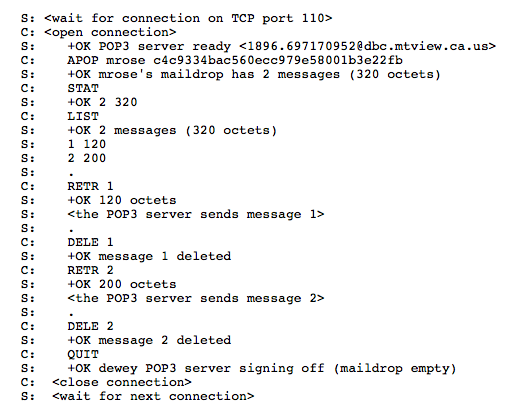
\includegraphics[scale=0.25]{images/pop3.png}
    \caption{Ancient horrors manifesting through the POP3 protocol.}
    \label{fig:how_pop3_works}
  \end{figure}
}

\nocite{*} % Include everything in the .bib file.

\bibliographystyle{plainnat}
\bibliography{presentation}

% that's all, folks
\end{document}
